\documentclass[conference]{IEEEtran}
\IEEEoverridecommandlockouts
% The preceding line is only needed to identify funding in the first footnote. If that is unneeded, please comment it out.
\usepackage{cite}
\usepackage{amsmath,amssymb,amsfonts, bm, bbm, amsthm}
\usepackage{algorithm}
% \usepackage{algorithmic}
\usepackage{algpseudocode}
\usepackage{graphicx}
\usepackage{textcomp}
\usepackage{xcolor}
\usepackage{tabularx}
\usepackage{caption}
\usepackage{subcaption}

\usepackage{thmtools, thm-restate}
\usepackage{hyperref}

\newtheorem{theorem}{Theorem}[section]
\newtheorem{corollary}{Corollary}[theorem]
\newtheorem{lemma}[theorem]{Lemma}

\theoremstyle{definition}
\newtheorem{definition}{Definition}[section]

\theoremstyle{plain}
\newtheorem{assumption}{Assumption}[section]

\theoremstyle{remark}
\newtheorem*{remark}{Remark}


\def\BibTeX{{\rm B\kern-.05em{\sc i\kern-.025em b}\kern-.08em
    T\kern-.1667em\lower.7ex\hbox{E}\kern-.125emX}}
\begin{document}

\title{EEC 289A Mini Lecture Paper Review\\
\vspace{0.5cm}
\textit{\large\textbf{\#23} Lumiere: A Space-Time Diffusion Model for Video Generation~\cite{bar2024lumiere} \\
\textbf{\#30} Sequential Modeling Enables Scalable Learning for Large Vision Models~\cite{bai2023sequential}}
}

\author{Chenye Yang}

\maketitle


\section{\textbf{\#23} Introduction}
The paper `Lumiere: A Space-Time Diffusion Model for Video Generation'~\cite{bar2024lumiere} addresses the critical challenge in video synthesis—creating realistic, diverse, and coherent motion. 
The authors introduce Lumiere, a text-to-video (T2V) diffusion model that synthesizes videos through a novel Space-Time U-Net (STUNet) architecture. 
Unlike existing models that generate distant keyframes followed by temporal super-resolution (TSR), which often leads to temporal inconsistencies, 
Lumiere processes the entire video duration in a single pass. 
This approach enables more globally coherent motion, facilitating a wide range of video content creation tasks such as image-to-video generation, video inpainting, and stylized video generation.
The pipeline of Lumiere is shown in Figure~\ref{fig:lumiere-pipeline}.
\begin{figure*}[!htbp]
    \centering
    \includegraphics[width=0.9\textwidth]{Lumiere-pipeline.png}
    \caption{The architecture of Lumiere.}
    \label{fig:lumiere-pipeline}
\end{figure*}


\section{\textbf{\#23} Method}
\subsection{Space-Time U-Net (STUNet) Architecture}
The core innovation of Lumiere is the Space-Time U-Net (STUNet) architecture, which diverges from traditional T2V models by handling both spatial and temporal dimensions simultaneously, shown in Figure~\ref{fig:STUNet-architecture}.
This architecture allows Lumiere to generate the entire video duration in a single pass, thereby ensuring global temporal coherence.
\begin{figure*}[!htbp]
    \centering
    \includegraphics[width=0.9\textwidth]{STUNet-architecture.png}
    \caption{The Space-Time U-Net (STUNet) architecture.}
    \label{fig:STUNet-architecture}
\end{figure*}

The STUNet is inspired by the 3D U-Net architecture used in volumetric biomedical data processing. It includes the following key components:
\begin{enumerate}
    \item Temporal Convolutions and Attention Mechanisms
    \item Inflation of Pre-trained T2I U-Net
    \item Spatial and Temporal Downsampling/Upsampling
\end{enumerate}

1)
Temporal Convolutions: These are integrated into the network to handle temporal information efficiently. They are designed to increase the non-linearities in the network while keeping computational costs manageable. Temporal convolutions are applied in all levels of the network except the coarsest level, where computational requirements are highest.
Temporal Attention: At the coarsest level, where the video representation is highly compressed, temporal attention layers are introduced. These layers help the model capture long-range dependencies in the temporal domain without significant computational overhead. Multiple temporal attention layers are stacked to enhance the model's expressiveness.


2)
The STUNet architecture is built by "inflating" a pre-trained text-to-image (T2I) U-Net model. This involves extending the 2D convolutional layers of the T2I model into 3D layers that handle both spatial and temporal dimensions.
The inflated architecture includes both convolution-based and attention-based inflation blocks. Convolution-based blocks perform space-time convolutions, while attention-based blocks apply temporal attention mechanisms.

3)
Downsampling: The input video signal is downsampled in both space and time, reducing its dimensionality and making the computation more tractable.
Upsampling: After processing the compact representation, the signal is upsampled back to its original resolution. This dual downsampling/upsampling approach ensures that the model can handle long video sequences efficiently.

\subsection{MultiDiffusion for Spatial Super-Resolution (SSR)}
To generate high-resolution videos, Lumiere incorporates a spatial super-resolution (SSR) cascade. 
Given the memory constraints of handling high-resolution video directly, Lumiere applies a technique called MultiDiffusion, which ensures temporal coherence across the entire video.
The MultiDiffusion process consists of the following steps: 
1) Segmented Processing. 
The SSR network processes the video in overlapping temporal segments. This segmentation prevents temporal boundary artifacts that can arise from processing non-overlapping segments.
Each segment of the video is processed independently, and the results are combined to form a coherent high-resolution output;
2) Optimization and Aggregation.
The outputs of the SSR network for each segment are reconciled through an optimization problem. This problem minimizes the differences between overlapping segments, ensuring a smooth transition across the entire video.
The solution involves linearly combining the overlapping predictions, producing a final video that maintains high visual quality and temporal consistency.

\subsection{Training and Fine-tuning}
Lumiere's model is trained using a large-scale video dataset, with the following training strategies:
1) Pre-training and Fine-tuning:
The model leverages a pre-trained T2I diffusion model, which provides a strong generative prior. The spatial layers of this T2I model are kept fixed, while the newly added temporal layers are trained on video data.
The temporal downsampling and upsampling modules are initialized to perform nearest-neighbor operations, ensuring that the model starts with a meaningful representation;
2) Conditional Generation:
Lumiere supports various forms of conditional video generation, including text-to-video, image-to-video, and video inpainting.
For image-to-video generation, the model conditions on the first frame of the video, with the rest of the frames generated to ensure temporal coherence.
For video inpainting, the model uses a binary mask to define regions that need to be animated, seamlessly integrating new content with the existing video.

\section{\textbf{\#23} Results}
The experiment results show Lumiere's ability to handle diverse application tasks such as text-to-video generation, image-to-video generation (Figure~\ref{fig:video-generation}), style-referenced generation, video inpainting, and cinemagraphs.
\begin{figure*}[!htbp]
    \centering
    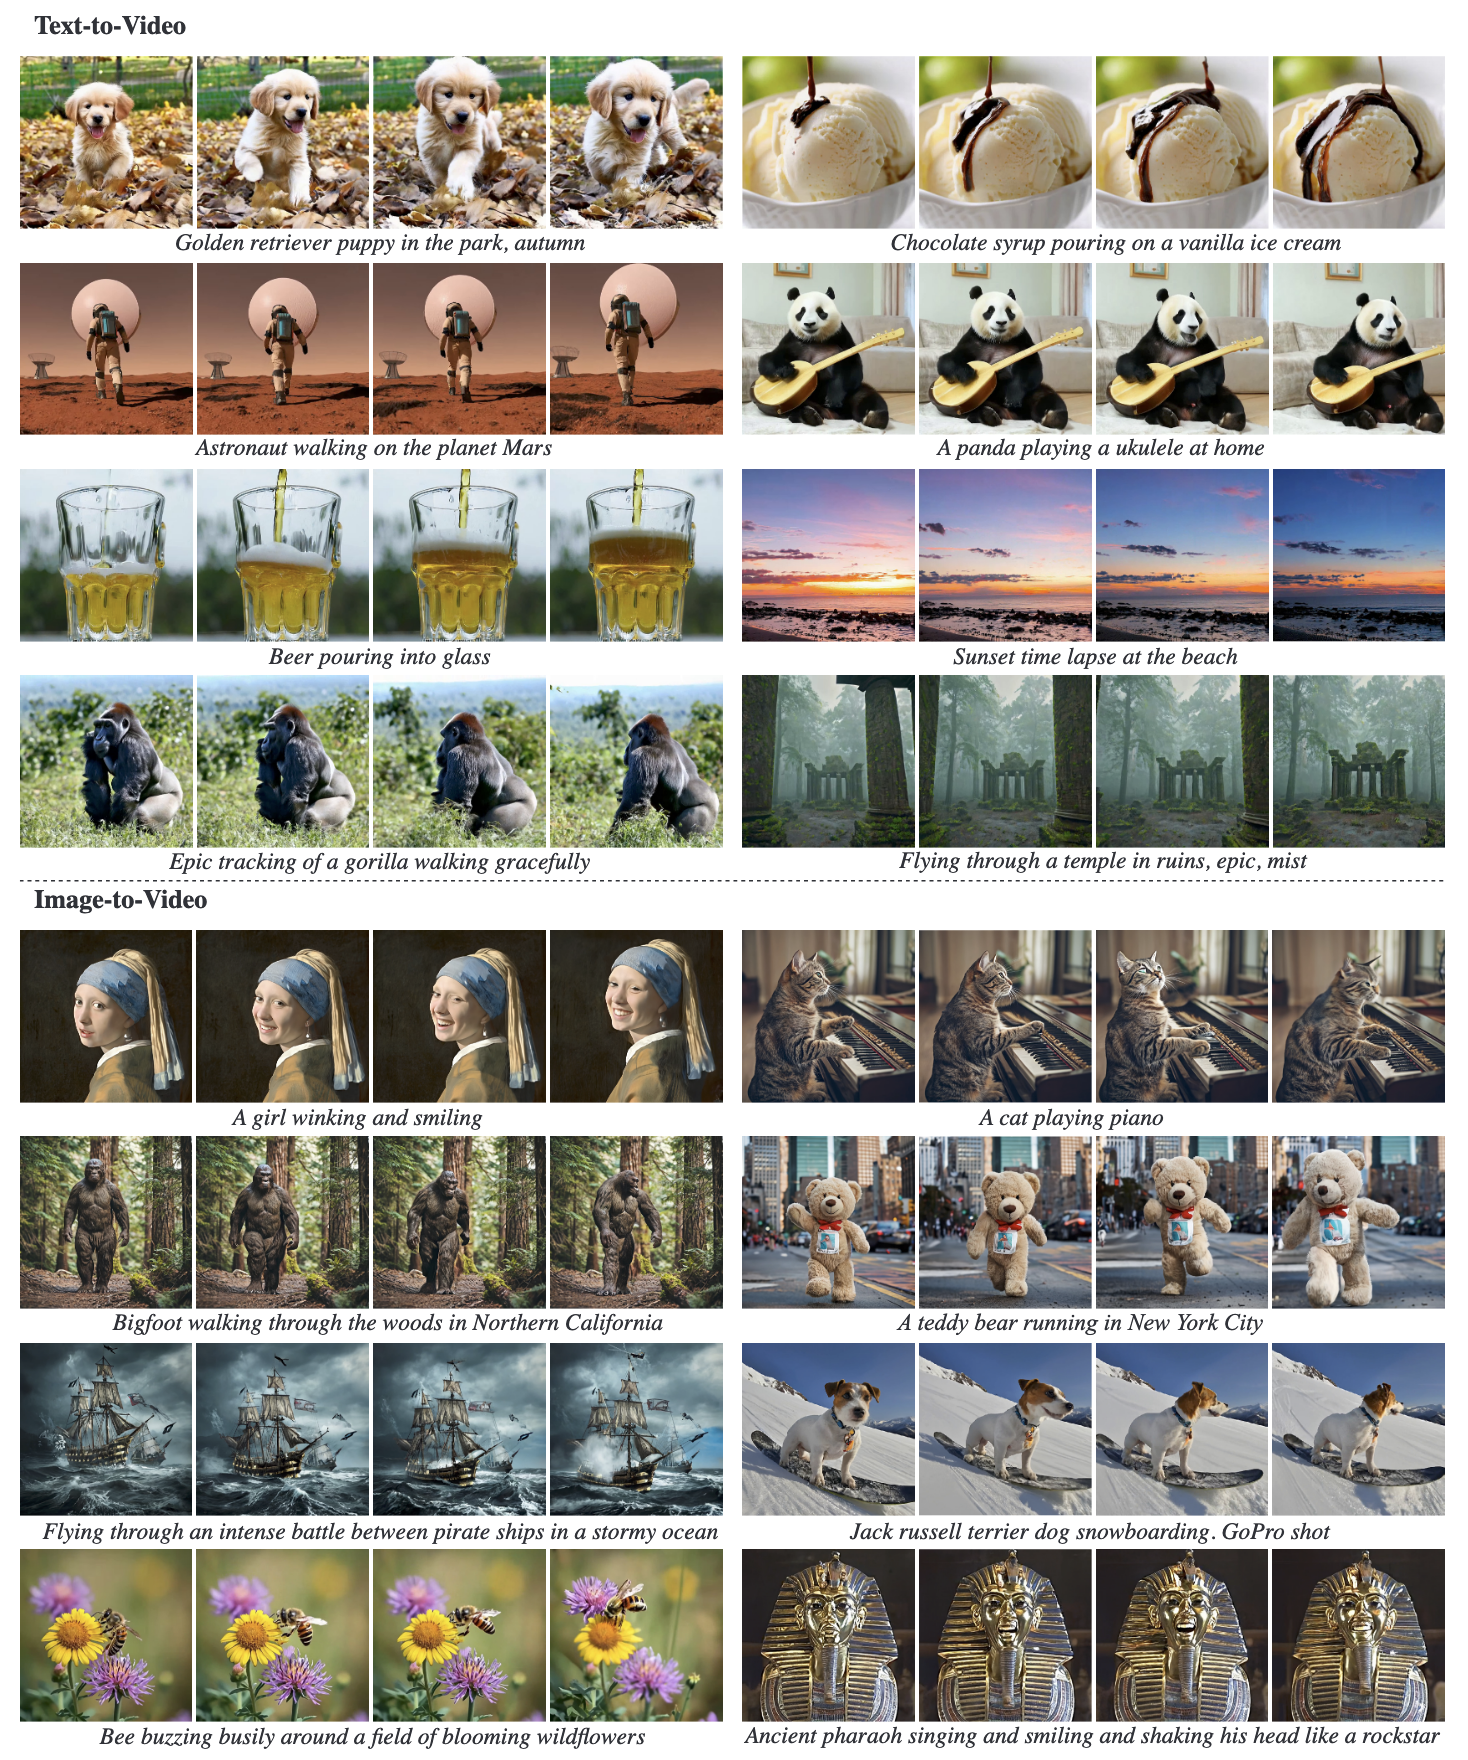
\includegraphics[width=0.9\textwidth]{video-generation.png}
    \caption{Video generation results of Lumiere.}
    \label{fig:video-generation}
\end{figure*}

The authors also did qualitative evaluation and quantitative evaluation against prominent T2V diffusion models, 
shown in Figure~\ref{fig:user-study} and Figure~\ref{fig:UCF101}, respectively.


\begin{figure*}
    \centering
    \includegraphics[width=0.9\textwidth]{User-study.png}
    \caption{Qualitative evaluation of Lumiere against other T2V models.}
    \label{fig:user-study}
\end{figure*}

\begin{figure}
    \centering
    \includegraphics[width=0.5\textwidth]{UCF101.png}
    \caption{Quantitative evaluation on UCF101 dataset, with metric Frechet Video Distance (FVD) and Inception Score (IS)}
    \label{fig:UCF101}
\end{figure}



\section{\textbf{\#30} Introduction}
The paper `Sequential Modeling Enables Scalable Learning for Large Vision Models'~\cite{bai2023sequential} presents a groundbreaking approach to developing Large Vision Models (LVMs) by leveraging sequential modeling techniques traditionally used in natural language processing. 
The core idea is to convert various forms of visual data, including images, videos, and annotated datasets, into a common sequential format called `visual sentences'. 
This unified format allows the application of transformer architectures for large-scale visual learning without relying on linguistic data. 
The authors aim to explore the scalability of vision models and their ability to handle a wide range of vision tasks through flexible prompting.








\section{\textbf{\#30} Method}
\subsection{Visual Sentence Representation}
The authors introduce the concept of `visual sentences', a common format to represent diverse visual data types (raw images, videos, semantic segmentations, depth reconstructions, etc.) as sequences. 
Each visual sentence is a sequence of visual tokens followed by an end-of-sentence (EOS) token. 
This representation facilitates the use of sequential modeling techniques for vision data, shown in 

\begin{figure}[!htbp]
    \centering
    \includegraphics[width=0.4\textwidth]{LVM-architecture.png}
    \caption{The architecture of Large Vision Models (LVMs).}
    \label{fig:LVM-architecture}
\end{figure}

The representation of visual sentences is achieved through the following steps:
1) Data Collection and Preparation:
The dataset, Unified Vision Dataset v1 (UVDv1), comprises 1.64 billion images/frames, including raw images, annotated images, unlabelled videos, and videos with annotations.
Visual sentences are created from these data sources, ensuring a diverse and comprehensive training dataset;
2) Tokenization:
A VQGAN model is used for tokenizing images. Each image is converted into a sequence of 256 vector-quantized tokens. The VQGAN encoder compresses the spatial dimensions, while the decoder reconstructs the image from tokens.
Tokenization is applied to individual images independently, allowing decoupling from downstream transformer training;
3) Sequential Modeling with Transformers:
The visual tokens from each image are concatenated to form a 1D sequence. These sequences are fed into an autoregressive transformer model to predict the next token, trained using a cross-entropy loss.
The model architecture follows a large transformer design similar to LLaMA, with parameter sizes ranging from 300 million to 3 billion.

\subsection{Training and Optimization}
The LVMs are trained using a single epoch over the UVDv1 dataset, with a context length of 4096 tokens. The training process employs the AdamW optimizer with specific hyperparameters to handle the vast amount of data efficiently.








\section{\textbf{\#30} Results}
The authors evaluate the performance of LVM on a wide range of aspects, inculding: training loss and scalability, performance on downstream tasks, dataset ablation study and sequential and analogy prompting. 
1) The training loss (perplexity) of LVMs of different sizes (300M, 600M, 1B, and 3B parameters) shows consistent improvement as the model size increases, indicating effective scalability. As depicted in Figure~\ref{fig:training-loss}, larger models achieve lower perplexity faster, demonstrating the model's ability to leverage larger parameter counts and more data efficiently.
2) The scalability of LVMs is further evaluated on four downstream tasks: semantic segmentation, depth estimation, surface normal estimation, and edge detection. Larger models consistently perform better across all tasks, as shown in Figure~\ref{fig:downstream}.
3) An ablation study investigates the contribution of different data components (unlabelled images, annotated images, videos, and videos with annotations) to the model's performance. Results in Figure~\ref{fig:data-ablation} demonstrate that each data component positively impacts downstream task performance, emphasizing the importance of dataset diversity.

The paper also compares the performance of LVMs with existing model (Visual Prompting) on various tasks such as foreground segmentation, single object detection, and colorization. The comparison, shown in Figure~\ref{fig:visual-prompting}, highlights that the LVMs outperform previous approaches, particularly in few-shot settings.

\begin{figure}[!htbp]
    \centering
    \includegraphics[width=0.3\textwidth]{training-loss.png}
    \caption{Training loss of LVMs with different parameter sizes.}
    \label{fig:training-loss}
\end{figure}

\begin{figure}[!htbp]
    \centering
    \includegraphics[width=0.5\textwidth]{downstream.png}
    \caption{Scalability of LVMs on downstream tasks.}
    \label{fig:downstream}
\end{figure}

\begin{figure}[!htbp]
    \centering
    \includegraphics[width=0.5\textwidth]{dataset-ablation.png}
    \caption{Ablation study on the impact of different data components on downstream task performance.}
    \label{fig:data-ablation}
\end{figure}

\begin{figure}
    \centering
    \includegraphics[width=0.5\textwidth]{visual-prompting.png}
    \caption{Comparison of LVMs with Visual Prompting on various vision tasks.}
    \label{fig:visual-prompting}
\end{figure}


\section{Conclusion}
Both Lumiere and the sequential modeling approach for LVMs contribute valuable advancements to the field of vision modeling.
\cite{bar2024lumiere} focus on improving the temporal coherence and quality of video generation, 
while \cite{bai2023sequential} aim to develop a scalable and flexible large vision model that can handle multiple vision tasks.







\bibliographystyle{unsrt}
\bibliography{bibliography}



\end{document}